\section{Цель работы}
Цеь работы -- найти приближенное значение определенного интеграла с требуемой точностью различными численными методами.
\section{Рабочие формулы используемых методов}
\begin{itemize}
	\item Метод прямоугольников
	      \[ \int_a^b f(x) \, dx \approx \sum_{i=1}^n f(\zeta_i) \Delta x_i \]
	\item Метод трапеций
	      \[ \int_a^b f(x) \, dx \approx 1/2 \sum_{i=1}^n h_i (y_{i-1} + y_i) \]
	\item Метод Симпсона
	      \[
		      \int_a^b f(x) \, dx \approx
		      \frac{h}{3} \Big[ y_0 + 4 (y_1 + y_3 + \ldots + y_{n-1}) + 2(y_2 + y_4 + \ldots + y_{n-2}) + y_n  \Big]
	      \]
	\item Правило Рунге
	      \[ I - I_{h/2} \approx \frac{I_{h/2} - I_{h}}{2^k - 1} \]
\end{itemize}

\section{Вычислительная часть задачи}
\[
	I = \int_2^4 (3 x^3 - 4 x^2 + 5 x - 16) \, dx
\]

Точное значение интеграла: \(\frac{310}{3} \approx 103.33\)
% https://www.wolframalpha.com/input?i2d=true&i=Integrate%5B3Power%5Bx%2C3%5D-4Power%5Bx%2C2%5D%2B5x-16%2C%7Bx%2C2%2C4%7D%5D

\subsection{По формуле Ньютона-Котеса}
\begin{align*}
	I & \approx \sum_{i=0}^6 f(x_i) c_n^i =                   \\
	  & =
	f(2) \cdot 41 \cdot 2 / 840 +
	f\left(\frac{7}{3}\right) \cdot 216 \cdot 2 / 840 +
	f\left(\frac{8}{3}\right) \cdot 27 \cdot 2 / 840 +
	f(3) \cdot 272 \cdot 2 / 840 +                            \\
	  & + f\left(\frac{10}{3}\right) \cdot 27 \cdot 2 / 840 +
	f\left(\frac{11}{3}\right) \cdot 216 \cdot 2 / 840 +
	f(4) \cdot 41 \cdot 2 / 840 =                             \\
	  & =
	0.20 + 6.17 + 1.66 + 28.50 + 4.33 + 49.60 + 12.89         \\
	  & \approx 103.33
\end{align*}

\[ \Delta I = 0 \quad (0 \%) \]

\subsection{Средние прямоугольники}
\begin{align*}
	I & \approx \sum_{i=0}^10 f(x_i) h =                                                                                  \\
    & = 0.2 \cdot \Big(f(2.10) + f(2.30) + f(2.50) + f(2.70) + \\ &+ f(2.90) + f(3.10) + f(3.30) + f(3.50) + f(3.70) + f(3.90)\Big) = \\
	  & = 0.2 \cdot \Big(4.64 + 10.84 + 18.38 + 27.39 + 38.03 + 50.43 + 64.75 + 81.12 + 99.70 + 120.62\Big) =                     \\
	  & = 0.2 \cdot 515.9 = 103.18                                                                                        \\
\end{align*}

\[ \Delta I = 0.1533 \quad (0.014\%) \]

\subsection{Метод трапеций}
\begin{align*}
	I & \approx 1/2 \sum_{i=0}^{10} h_i (y_{i-1} + y_i) =                                                                                        \\
    & = 2/10 \cdot \Big(1/2 \cdot (f(2.00) + f(4.00)) + f(2.20) + \\ &+ f(2.40) + f(2.60) + f(2.80) + f(3.00) + f(3.20) + f(3.40) + f(3.60) + f(3.80)\Big) = \\
    & = 2/10 \cdot \Big(1/2 \cdot (2.00 + 132.00) + 7.58 + 14.43 + 22.69 \\ &+ 32.50 + 44.00 + 57.34 + 72.67 + 90.13 + 109.86\Big) =                       \\
	  & = 103.64
\end{align*}
Погрешность: \[ \Delta I \approx 0.31 \quad (0.3 \%)  \]

\subsection{Метод Симпсона}

\begin{align*}
	I & \approx 123                                                                                                                                                                                                          \\
    & = 2/10 \cdot 1/3 \cdot \Big(1/2 (f(2.00) + f(4.00)) + 4 \cdot f(2.20) + 2 \cdot f(2.40) + 4 \cdot f(2.60) + \\ &+ 2 \cdot f(2.80) + 4 \cdot f(3.00) + 2 \cdot f(3.20) + 4 \cdot f(3.40) + 2 \cdot f(3.60) + 4 \cdot f(3.80)\Big) = \\
    & = 2/10 \cdot 1/3 \cdot \Big(1/2 \cdot (2.00 + 132.00) + 4 \cdot 7.58 + 2 \cdot 14.43 + 4 \cdot 22.69 + \\ &+ 2 \cdot 32.50 + 4 \cdot 44.00 + 2 \cdot 57.34 + 4 \cdot 72.67 + 2 \cdot 90.13 + 4 \cdot 109.86\Big) =                 \\
	  & = 103.33
\end{align*}

\[ \Delta I = 0 \quad (0\%) \]

\section{Программная часть задачи}
\inputminted[breaklines]{Python}{./solution.py}

\begin{figure}[H]
	\centering
	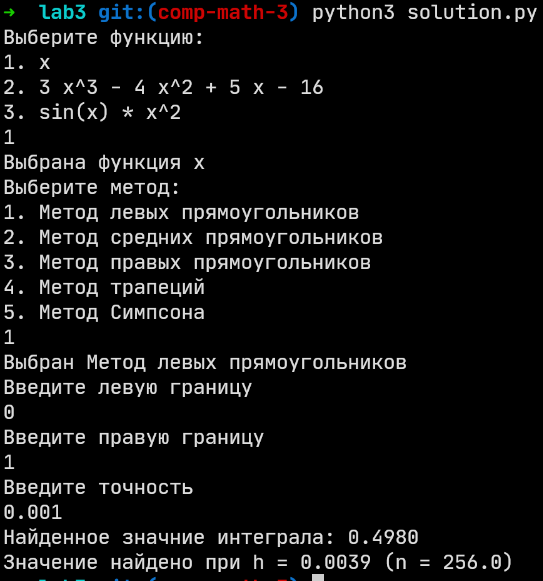
\includegraphics[width=0.5\textwidth]{./img/test1.png}
\end{figure}
\begin{figure}[H]
	\centering
	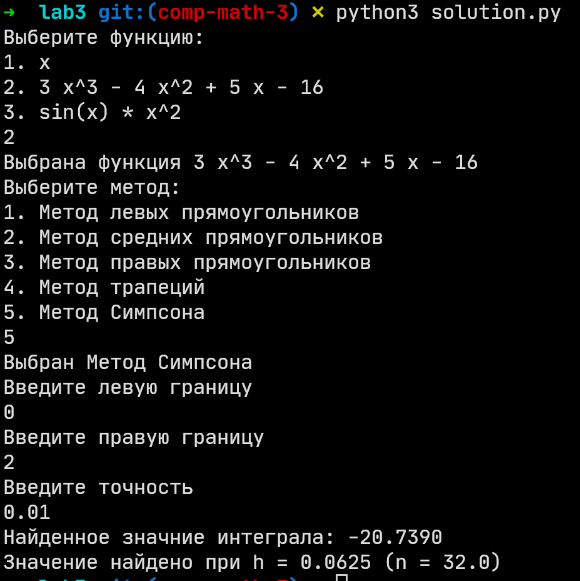
\includegraphics[width=0.5\textwidth]{./img/test2.png}
\end{figure}
\begin{figure}[H]
	\centering
	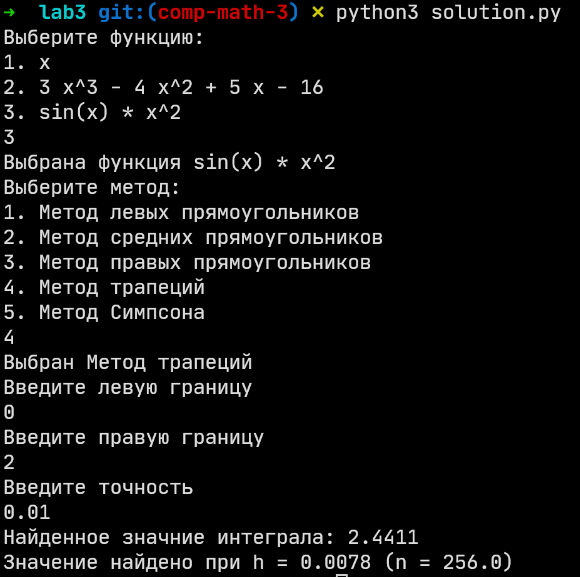
\includegraphics[width=0.5\textwidth]{./img/test3.png}
\end{figure}

\section{Вывод}
При выполнении данной лабораторной работой мною были
изучены такие методы численного интегрирования как
метод прямоугольников, метод трапеций и метод Симпсона.
Эти методы были реализованы мною на языке программирования
Python.
